%*******************************************************************************
% Example chapter file for books, Copyright A K Peters, Ltd.
%*******************************************************************************
\chapter{Depth of Field with Bokeh Rendering}{Charles de Rousiers and Matt Pettineo}
\label{BokehRendering}

%-------------------------------------------------------------------------------
\section{Introduction}

In order to increase realism and immersion, current games make frequent use of depth of field to simulate lenticular phenomena. Typical implementations use blur based approaches to simulate a camera’s circle of confusion out-of-focus parts of a scene. While such approaches give reasonable results, important features are still missing. In particular, real cameras produce a typical effect that photographers call bokeh (blur in Japanese) appearing at contrasted locations of the final image. Bokeh reveals itself as  bright blurry spots whose shape depends on the camera’s aperture (typically, a circle, a pentagon, or octagon). 

Current and upcoming DirectX11 engines (i.e. Cry engine, Unreal Engine, ...) have recently shown a particular interest for such effects as attested by their most recent demos. Still, it  remains an up-coming technology and precise implementation details are not available yet.

Explicitly drawing the aperture’s shape with quad rendering for every pixel would be rather inefficient. Instead, we propose an hybrid method, mixing previous blur based approaches with quad rendering. Our method selects high contrasted points, and for each of them, renders a quad with an aperture texture. In order to achieve high performance, we use both atomic counters, image texture for random memory access, and indirect draw command for avoiding CPU / GPU synchronizations. This efficient OpenGL 4.2 implementation allows to draw thousands of aperture’s shape at high frame-rate and ensures the temporal coherency of the rendered bokeh.

%-------------------------------------------------------------------------------
\section{Depth of Field Phenomemon}\label{Derousiers:DOFPhenomenon}
Depth of field is an important effect to convey realism, especially in opened scenes, with a large field of view. Traditional real-time applications use pinhole camera, which have an infinite depth of field. On the contrary, real camera use thin lens which introduces a limited depth of field. Objects outside this depth of field appear blurred on the final image. Objects inside this depth of field appear sharp, see Figure~\ref{DeRousiers:focus}.

	\begin{figure}[htb]\centering
	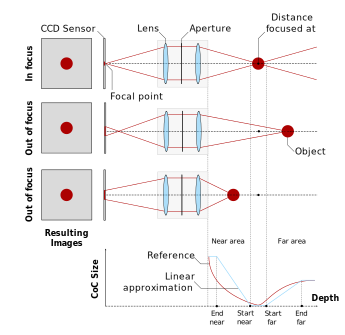
\includegraphics[width=\textwidth]{focus}
	\caption{An object appears blurred depending of its positions in the camera's field of view. 
If an object is in the focused area, then it appear clearly. Othewise, it appears blurred. }
	\label{DeRousiers:focus}
	\end{figure}


The "bluriness" of an object is defined by its circle of confusion (\coc). The size of this \coc depends on the distance to the focused area. Further a object is from focused area, blurier it appears. The \coc size is not linearly dependent from this distance. It increase faster in the unfocused foreground area than in the unfocused background area, see Figure~\ref{Derousiers:focus}. \coc depends on focal distance and lens' size. It is not obvious how to set up these two parameters to obtain the desire depth of field. This is why we use a linear approximation as proposed by~\cite{Hammon07}, see Figure~\ref{DeRousiers:focus}.

	\begin{figure}[htb]\centering
	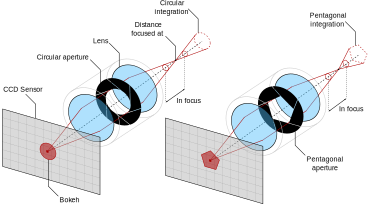
\includegraphics[width=\textwidth]{camera}
	\caption{Aperture's shape of a camera. Aperture's shape modifies pixel integration, and changes bokeh shape }
	\label{DeRousiers:camera}
	\end{figure}

Additionaly, real cameras have an aperture which is in charge of letting light come in when a photograph is taken\footnote{If an object or the camera moves during aperture opening, objects will appear blured : it is the motion blur.}. Aperture shape impact directly the final image aspect. Each point out of focus is convolved with the aperture shape. Changing the aperture shape, modify the final image, see Figure~\ref{DeRousiers:camera}.

While it is hard to see bokeh for low constrated area, bokehs appear clearly for highly constrasted point. We use this observation as an heuristique to determine where bokehs have to be drawn.

%-------------------------------------------------------------------------------
\section{Relative Work}\label{Derousiers:RelativeWork}

Several methods have been proposed during the last decade to approximate efficiently depth of field effect. But those methods use gaussian blur or heat diffusion to process unfocused areas~\cite{Kosloff07,Hammon07} and are not able to reproduce bokeh effects.

The earlier approach from Krivanek~\cite{Krivanek03} use sprite splatting for rendering depth of field effect. While this brute force method would allow to render bokehs, it is quite inefficient due to overdraw. Video game industry has shown a recent interest for bokeh effects~\cite{Sousa11,Futurmark11,Mittring11}. While implementation details are uncovered, all those methods seem use a sprite for each pixel as Krivanek. However those techniques use clever tricks to optimize performances (hierarchical rasterisation,...). 

A recent approach proposed by White~\cite{White11} reproduces pentagonal bokeh efficiently using several directional blur passes. While efficient, this method does not support arbitrary bokeh shape.

%-------------------------------------------------------------------------------
\section{Algorithm}
We observe that only high constrasted points produce distinct bokehs. We use this heuristic to detect bokeh positions in screen space~\cite{Pettineo11} and render final bokehs by splatting textured quad at those locations.

\subsection{Overview}
Our approch is divide into four passes. The first pass computes the \coc size for each pixel based on its depth value and output a linear depth buffer\footnote{If you already have a linear depth buffer as input, you can merge together the first two passes.}. Then, the second pass compute the contrast of the current pixel and append its position, \coc size, and averaged color to a buffer, if this constrast is enough. During the third pass, blur-based depth of field is computed with one of the previous methods (gaussian blur,...). Finally, the last pass splats textured quad at bokeh positions.

	\begin{figure}[htb]\centering
	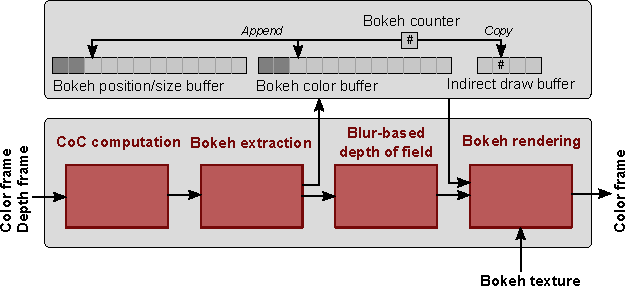
\includegraphics[width=\textwidth]{pipeline}
	\caption{Overview of the pipeline.}
	\label{YourName:fig1}
	\end{figure}

In order to ensure high performances, CPU/GPU synchronization has to be avoided. We use an indirect draw command which read from a GPU buffer how many bokeh has to be drawn. This way, the number of detected bokehs is never read back by the CPU.

\subsection{Circles of confusion computation}
Settings field of view with focal length is not easy.
We define two areas where geometry is unfocused : a foreground area and a background area. Both areas are delimited with a near and far depth values, see Figure~\ref{DeRousiers:focus}. Blur amout is linearly interpolated between those bounds. It allows a easy and intuitive way to set up field of view.

$$
	CoC = \frac{Z_{pixel} - Z_{near} }{ Z_{far} - Z_{near} }
$$

This way the \coc size is normalized between [0,1]. An extra parameter \codecmd{MaxRadius} determines a posterori what is final size of the blur. This lets artists to play with, in order to achieve the desired appearance and also balances performances (lesser the \codecmd{MaxRadius} is, greater the performances are).


\subsection{Bokeh detection}
This pass aims to detect pixels which will generate \bokehs. To detect them we use the following heuristic : \emph{an highly constrasted pixel in a given neighborhood will generate a bokeh}. We compare the current pixel luminance $L_{pixel}$ to its neighborhood luminance $L_{neigh}$. If the difference $L_{pixel}-L_{neigh}$ is greater than the threshold \codecmd{LumThreshold}, then the current pixel is registered as a bokeh. Pixels detected as bokeh are sparse. Storing them into a render target texture would be a waste of space and reading them back would be a waste of time due to their no-coherency in space. To address this problem, we use the \opengl \codecmd{ImageBuffer}s in combinaison with \codecmd{AtomicCounter}. This allows us to built a vector in which we append detected bokehs parameters. \codecmd{ImageBuffer}s have to be preallocated with a given size (\ie the maximum number of bokehs which can be display on screen). The \codecmd{AtomicCounter} stores the number of appended bokehs. Its current value indicades the next free cells in the \codecmd{ImageBuffers} vector. Two ImageBuffer are used to store \coc size, position, and color of the registered bokeh. 


\subsection{Blur-based depth of field}
Several approach are possible for this pass. We refer readers to previous work for this step. Nevertheless, here a short sum up of main approaches :
\begin{itemize}
	\item Do a constant kernel gaussian blur at various resolutions and apply a linear interpolation to blend them according to \coc size.
	\item Do a Poisson disc sampling with a radius adapted to \coc size~\footnote{A random rotation can be applied to Poisson sampling pattern for transforming aliasing into noise.}.
	\item Do a large bilateral filtering and rejecting invalid pixel~\footnote{For implementation details, we refer the reader to the code sample. Thsi approach offers a good compromise between quality and performances. However it need large radius. A \opencl implementation would allow better performances, since shared memory can be used to cache texture fetches.}.
\end{itemize}


\subsection{Bokeh rendering}
In order to avoir CPU/GPU synchonization, we use an indirect drawing command \codecmd{glDrawArraysIndirect}. This command draw instances of a given VBO/VAO. The number of instance is specified into a buffer located on the GPU memory. The buffer can be updated from the CPU or updated from the GPU. For performances concerns, we update this buffer from the GPU during the second pass. 

We use this command in combinaison point VAO. The instanced points are translated into the vertex shader to be located at bokeh position. The position is read from BokehPositionBuffer by using the built-in \codecmd{gl\_InstanceID} index. Each point is expanded in a quad into the geometry shader. The size of the quad is adaped to bokeh size (also store into BokehPositionBuffer). Finally, the fragment shader applies the bokeh alpha-texture onto the quad and multiply it by the bokeh color (store into BokehColorBuffer).

%-------------------------------------------------------------------------------
\section{Results}

\subsection{Rendering}
	\begin{figure}[htb]\centering
	
\includegraphics[width=\textwidth]{todo}
	\caption{Rendering 1.}
	\label{YourName:fig1}
	\end{figure}

	\begin{figure}[htb]\centering
	
\includegraphics[width=\textwidth]{todo}
	\caption{Rendering 2.}
	\label{YourName:fig1}
	\end{figure}

\subsection{Performances}
	\begin{figure}[htb]\centering
	
\includegraphics[width=\textwidth]{todo}
	\caption{Performances.}
	\label{YourName:fig1}
	\end{figure}

%-------------------------------------------------------------------------------
\section{Discussion}
One may concerns about temporal coherency for this approach. Just as all other approach, we base our approch of the final color buffer. If sub-pixel aliasing is handled properly by previous rendering steps, our approach is stale and bokehs are coherent frame-to-frame. In case of sub-pixel aliasing, our method exhib same limitation as all previous methods, and bokehs may flicked.

Our methods need pre-allocated buffers for storing bokeh position and color information. Hence, a maximum number of bokehs has to be specified. If this number is too low artifacfs may arise, like bokeh popping. If this number is too large, GPU memory usage is wasted. Thus, the right maximal number as to be according the type of scenes displayed.

%-------------------------------------------------------------------------------
\section{Conclusion}
We have presented an efficient implementation for rendering depth of field effect that produces bokehs. This method allow to combine efficient blur-approach with bokeh reproduction. We use an heuristique to identify pixels that produce distinct bokeh and render them with textured quads. This implementation avoids CPU/GPU synchronisation by calling indirect draw commands. These command read directly the number of instances to draw on GPU, without back reading from the CPU.


\textbf{Future work:} While this approach provides good results, several improvments could be done for improving performances. Especially, atomic-counter are not super fast. By dividing screen into four parts, each part having an atomic counter, let concurrent operation would produce a the same time. Large \coc size require to rasterize quad on large portion of the screen. Using the hierarchical rasterization proposed in~\cite{Futurmark11} would also improve performances.



\begin{lstlisting}[language=C++,float={htb},caption={Initialization and drawing for extracting bokehs.},label={YourName:bokehextraction}]


		// Indirect buffer definition
		struct DrawArraysIndirectCommand
		{
			GLuint count;
			GLuint primCount;
			GLuint first;

			GLuint reservedMustBeZero;
		};

		...

		// Create atomic counter
		GLuint indirectBufferID;

		glGenBuffers(1,&indirectBufferID);
		glBindBuffer(GL_DRAW_INDIRECT_BUFFER,indirectBufferID);
		DrawArraysIndirectCommand indirectCmd;
		indirectCmd.count              = 1;
		indirectCmd.primCount          = 6;
		indirectCmd.first              = 0;
		indirectCmd.reservedMustBeZero = 0;

		glBufferData(GL_DRAW_INDIRECT_BUFFER,sizeof(DrawArraysIndirectCommand),&indirecCmd,GL_DYNAMIC_DRAW);

		// Create a texture proxy for the indirect buffer
		glGenTextures(1, &bokehCountTexID);
		glBindTexture(GL_TEXTURE_BUFFER, bokehCountTexID);
		glTexBuffer(GL_TEXTURE_BUFFER, GL_R32UI, pointIndirectBuffer.id);


		// Create position and color textures with a GL_RGBA32F inner format

		...

		// Bind atomic counter
		glActiveTexture(GL_TEXTURE0 + bokehCountTexUnit);
		glBindTexture(GL_TEXTURE_BUFFER, bokehCountTexID);

		glBindImageTexture(bokehCountTexUnit,bokehCountTexID,0,false,0,GL_READ_WRITE,GL_R32UI);

		// Bind position image buffer
		glActiveTexture(GL_TEXTURE0 + bokehPosTexUnit);
		glBindImageTexture(bokehPosTexUnit,bokehPosTex.id,0,false,0,GL_READ_WRITE,GL_RGBA32F);

		// Bind color image buffer

		glActiveTexture(GL_TEXTURE0 + bokehColorTexUnit);
		glBindImageTexture(bokehColorTexUnit,bokehColorTex.id,0,false,0,GL_READ_WRITE,GL_RGBA32F);

		DrawSceenQuad();
\end{lstlisting}


\begin{lstlisting}[language=GLSL,float={htb},caption={Fragment shader for extracting bokehs.},label={YourName:listing1}]
	#version 420

	// Bokeh counter, position (x,y,z,size), and color
	layout(size1x32) coherent uniform uimage1D 	BokehCountTex;
	layout(size4x32) coherent uniform  image1D 	BokehPosTex;
	layout(size4x32) coherent uniform  image1D 	BokehColorTex;


	// Constrast threshold
	uniform float lumThreshold;

	...

	float sizeCenter; // Current CoC size

	vec3 colorCenter; // Current pixel color
	vec3 colorNeighs; // Average color of the neighborhood

	// Append pixel whose constrast is greater than the user's threshold
	float lumNeighs = dot(colorNeighs, vec3(0.299f, 0.587f, 0.114f));
	float lumCenter = dot(colorCenter, vec3(0.299f, 0.587f, 0.114f));
	if((lumCenter-lumNeighs)>lumThreshold)
	{
		int current = int(imageAtomicAdd(BokehCountTex, 1, 1));
		imageStore(BokehPosTex,current,vec4(gl_FragCoord.x,gl_FragCoord.y,gl_FragCoord.z,sizeCenter));
		imageStore(BokehColorTex,current,vec4(colorCenter,1));
	}
\end{lstlisting}




\begin{lstlisting}[language=C++,float={htb},caption={Your caption.},label={YourName:listing1}]

	// Create point VBO
	GLuint pointVboID;
	glm::vec3 defaultPosition(0,0,0);

	glGenBuffers(1,&pointVboID);
	glBindBuffer(GL_ARRAY_BUFFER,pointVboID);
	glBufferData(GL_ARRAY_BUFFER,sizeof(glm::vec3),&defaultPosition,GL_STATIC_DRAW);

	// Create point VAO
	GLuint pointVaoID;
	glGenVertexArrays(1, &pointVaoID);

	glBindVertexArray(pointVaoID);
	glVertexAttribPointer(semantic::PositionLocation,3, GL_RGB,false,GL_FLOAT,GLF_BUFFER_OFFSET(_offset));
	glEnableVertexAttribArray(semantic::PositionLocation);
	glBindBuffer(GL_ARRAY_BUFFER, 0);
	glBindVertexArray(0);

	...


	glMemoryBarrier(GL_ALL_BARRIER_BITS);
	glUseProgram(bokehRenderingProgramID);

	glActiveTexture(GL_TEXTURE0 + bokehShapeTexUnit);
	glBindTexture(GL_TEXTURE_1D,bokehShapeTexID);
	glActiveTexture(GL_TEXTURE0 + bokehColorTexUnit);

	glBindTexture(GL_TEXTURE_1D,bokehColorTexID);
	glActiveTexture(GL_TEXTURE0 + bokehPosTexUnit);
	glBindTexture(GL_TEXTURE_1D,bokehPosTexID);

	glBindVertexArray(pointVaoID);
		glBindBuffer(GL_DRAW_INDIRECT_BUFFER,indirectBufferID);
		glDrawArraysIndirect(GL_POINTS,NULL);

		glBindBuffer(GL_DRAW_INDIRECT_BUFFER,0);
	glBindVertexArray(0);

\end{lstlisting}


\begin{lstlisting}[language=C++,float={htb},caption={Vertex shader for rendering bokeh.},label={YourName:listing1}]
#version 420

uniform vec2      PixelScale;    // (1/xResolution,1/yResolution)
uniform sampler1D BokehPosTex;   // (x,y,z,scale)
uniform sampler1D BokehColorTex;
in vec3           Position;

out float         Radius;
out vec4          Color;

int main()
{
	vec3 pos     = texelFetch(BokehPosTex,gl_InstanceID,0).xyzw;
	Radius       = pos.w;

	Color        = texelFetch(BokehColorTex,gl_InstanceID,0);
	gl_Position	 = vec4( (Position.xy+pos.xy)*PixelScale,pos.z,1);
}
\end{lstlisting}

\begin{lstlisting}[language=GLSL,float={htb},caption={Geometry shader for rendering bokeh.},label={YourName:listing1}]
#version 420


uniform mat4     Transformation;
uniform vec2     PixelScale;
in  float        Radius[1];
in  vec4         Color[1];
out vec4         Radiance;
out vec2         TexCoord;

layout(points)   in;
layout(triangle_strip, max_vertices = 6) out;

void main()
{
	gl_Layer     = 0;
	vec4 offsetx = vec4(PixelScale.x*Radius[0],0,0,0);

	vec4 offsety = vec4(0,PixelScale.y*Radius[0],0,0);
	Radiance     = Color[0];

	// First triangle
	gl_Position = Transformation * ( gl_in[0].gl_Position-offsetx-offsety);
	TexCoord    = vec2(0,0);
	EmitVertex();


	gl_Position = Transformation * ( gl_in[0].gl_Position+offsetx-offsety);
	TexCoord    = vec2(1,0);
	EmitVertex();

	gl_Position = Transformation * ( gl_in[0].gl_Position+offsetx+offsety);
	TexCoord    = vec2(1,1);

	EmitVertex();
	EndPrimitive();

	// Second triangle
	gl_Position = Transformation * ( gl_in[0].gl_Position-offsetx-offsety);
	TexCoord    = vec2(0,0);
	EmitVertex();


	gl_Position = Transformation * ( gl_in[0].gl_Position+offsetx+offsety);
	TexCoord    = vec2(1,1);
	EmitVertex();

	gl_Position = Transformation * ( gl_in[0].gl_Position-offsetx+offsety);
	TexCoord    = vec2(0,1);

	EmitVertex();
	EndPrimitive();
}
\end{lstlisting}

\begin{lstlisting}[language=GLSL,float={htb},caption={Fragment shader for rendering bokeh.},label={YourName:listing1}]
#version 420


uniform sampler2D    BokehShapeTex; // Bokeh shape texture
uniform float        Attenuation;   // Factor for attenuating bokeh borders
in  vec4             Radiance;
in  vec2             TexCoord;
out vec4             FragColor;


void main()
{
	// Add an attenuation function in order to avoid hard edge on the 
	// aperture shape
	float val = textureLod(BokehShapeTex,TexCoord,0).x;
	float att = clamp(length(2.f*(TexCoord-vec2(0.5))),0.f,1.f);
	att       = 1.f - pow(att,Attenuation);
	FragColor = vec4(Radiance.xyz * val * att,Radiance.w);
}
\end{lstlisting}



%-------------------------------------------------------------------------------
\bibliographystyle{akpbib}
\bibliography{BokehRendering}











